\documentclass{standalone}
\usepackage{tikz}
\usetikzlibrary{patterns, positioning}

\begin{document}
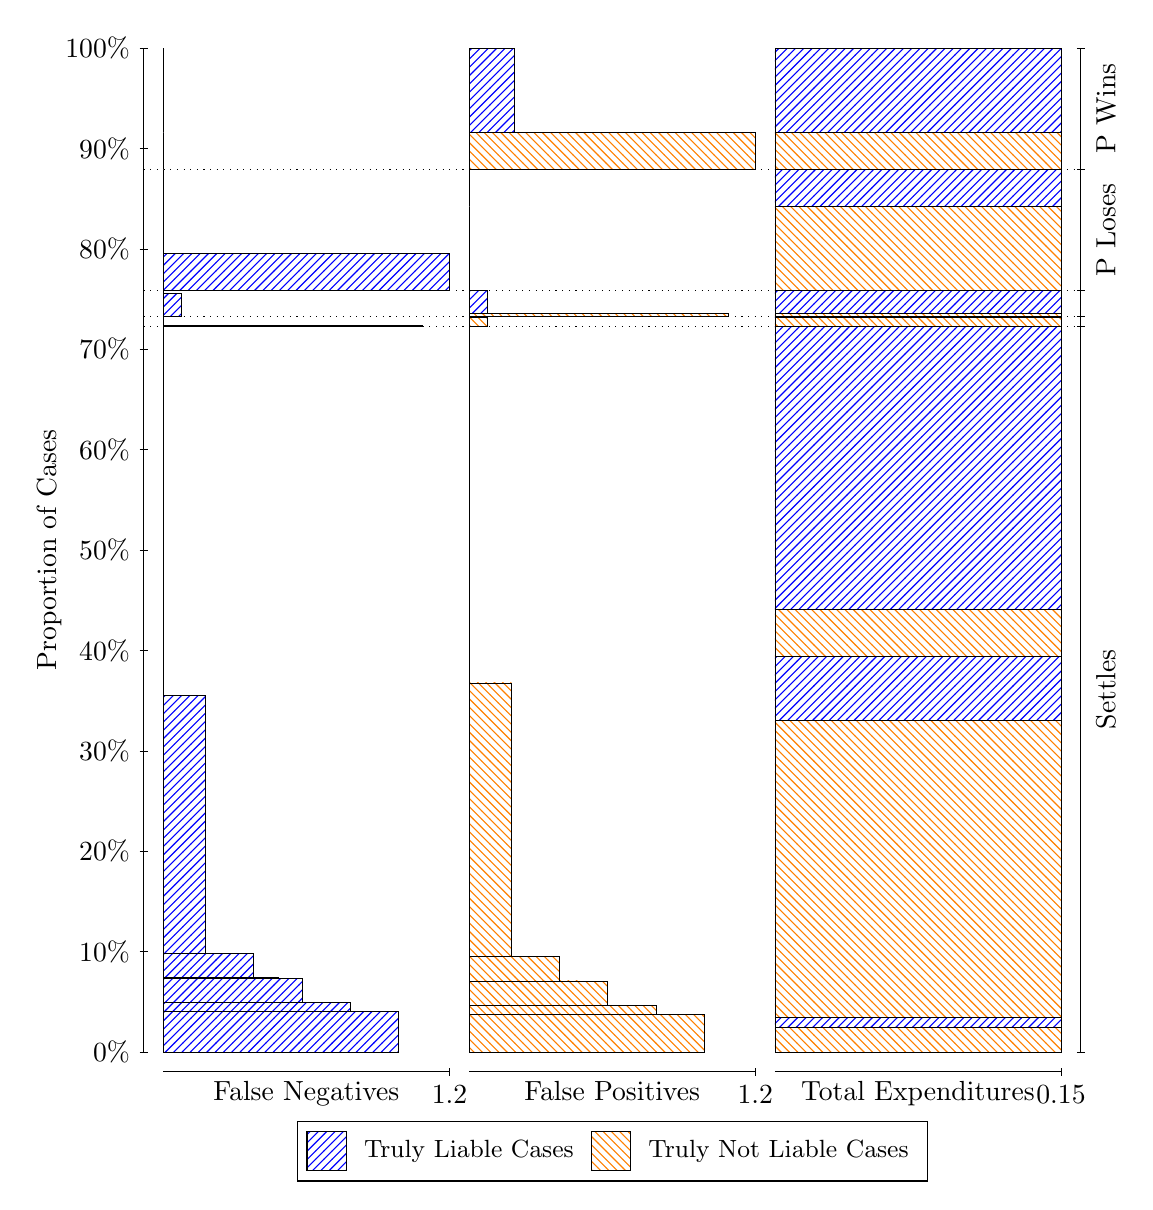
\begin{tikzpicture}
\draw[black, very thin] (1.5,1.75) -- (1.5,14.5);
\node[rotate=90, anchor=center] at (0.3, 8.125) {Proportion of Cases};
\draw[black, very thin] (1.45,1.75) -- (1.55,1.75);
\node[anchor=east] at (1.45, 1.75) {0\%};
\draw[black, very thin] (1.45,3.025) -- (1.55,3.025);
\node[anchor=east] at (1.45, 3.025) {10\%};
\draw[black, very thin] (1.45,4.3) -- (1.55,4.3);
\node[anchor=east] at (1.45, 4.3) {20\%};
\draw[black, very thin] (1.45,5.575) -- (1.55,5.575);
\node[anchor=east] at (1.45, 5.575) {30\%};
\draw[black, very thin] (1.45,6.85) -- (1.55,6.85);
\node[anchor=east] at (1.45, 6.85) {40\%};
\draw[black, very thin] (1.45,8.125) -- (1.55,8.125);
\node[anchor=east] at (1.45, 8.125) {50\%};
\draw[black, very thin] (1.45,9.4) -- (1.55,9.4);
\node[anchor=east] at (1.45, 9.4) {60\%};
\draw[black, very thin] (1.45,10.675) -- (1.55,10.675);
\node[anchor=east] at (1.45, 10.675) {70\%};
\draw[black, very thin] (1.45,11.95) -- (1.55,11.95);
\node[anchor=east] at (1.45, 11.95) {80\%};
\draw[black, very thin] (1.45,13.225) -- (1.55,13.225);
\node[anchor=east] at (1.45, 13.225) {90\%};
\draw[black, very thin] (1.45,14.5) -- (1.55,14.5);
\node[anchor=east] at (1.45, 14.5) {100\%};

\draw[black, very thin] (13.4,1.75) -- (13.4,14.5);
\draw[black, very thin] (13.35,1.75) -- (13.45,1.75);
\node[anchor=west] at (13.35, 1.75) {};
\draw[black, very thin] (13.35,10.964) -- (13.45,10.964);
\node[anchor=west] at (13.35, 10.964) {};
\draw[black, very thin] (13.35,11.09) -- (13.45,11.09);
\node[anchor=west] at (13.35, 11.09) {};
\draw[black, very thin] (13.35,11.422) -- (13.45,11.422);
\node[anchor=west] at (13.35, 11.422) {};
\draw[black, very thin] (13.35,12.959) -- (13.45,12.959);
\node[anchor=west] at (13.35, 12.959) {};
\draw[black, very thin] (13.35,14.5) -- (13.45,14.5);
\node[anchor=west] at (13.35, 14.5) {};

\draw[black, very thin, pattern color=blue, pattern=north east lines] (1.75,1.75) rectangle (4.7332,2.2606);
\draw[black, very thin, pattern color=blue, pattern=north east lines] (1.75,2.2606) rectangle (4.4272,2.2647);
\draw[black, very thin, pattern color=blue, pattern=north east lines] (1.75,2.2647) rectangle (4.1212,2.378);
\draw[black, very thin, pattern color=blue, pattern=north east lines] (1.75,2.378) rectangle (3.8153,2.3829);
\draw[black, very thin, pattern color=blue, pattern=north east lines] (1.75,2.3829) rectangle (3.5093,2.6849);
\draw[black, very thin, pattern color=blue, pattern=north east lines] (1.75,2.6849) rectangle (3.2033,2.693);
\draw[black, very thin, pattern color=blue, pattern=north east lines] (1.75,2.693) rectangle (2.8974,3.0021);
\draw[black, very thin, pattern color=blue, pattern=north east lines] (1.75,3.0021) rectangle (2.5914,3.0029);
\draw[black, very thin, pattern color=blue, pattern=north east lines] (1.75,3.0029) rectangle (2.2854,6.2752);
\draw[black, very thin, pattern color=orange, pattern=north west lines] (1.75,6.2752) rectangle (1.75,10.964);
\draw[black, very thin, pattern color=blue, pattern=north east lines] (1.75,10.964) rectangle (5.0391,10.975);
\draw[black, very thin, pattern color=orange, pattern=north west lines] (1.75,10.975) rectangle (1.75,11.09);
\draw[black, very thin, pattern color=blue, pattern=north east lines] (1.75,11.09) rectangle (1.9795,11.387);
\draw[black, very thin, pattern color=orange, pattern=north west lines] (1.75,11.387) rectangle (1.75,11.422);
\draw[black, very thin, pattern color=blue, pattern=north east lines] (1.75,11.422) rectangle (5.3833,11.892);
\draw[black, very thin, pattern color=orange, pattern=north west lines] (1.75,11.892) rectangle (1.75,12.959);
\draw[black, very thin, pattern color=orange, pattern=north west lines] (1.75,12.959) rectangle (1.75,13.428);
\draw[black, very thin, pattern color=blue, pattern=north east lines] (1.75,13.428) rectangle (1.75,14.5);
\draw[black, very thin, pattern color=orange, pattern=north west lines] (5.6333,1.75) rectangle (8.6165,2.2291);
\draw[black, very thin, pattern color=orange, pattern=north west lines] (5.6333,2.2291) rectangle (8.3105,2.2307);
\draw[black, very thin, pattern color=orange, pattern=north west lines] (5.6333,2.2307) rectangle (8.0046,2.3429);
\draw[black, very thin, pattern color=orange, pattern=north west lines] (5.6333,2.3429) rectangle (7.6986,2.3464);
\draw[black, very thin, pattern color=orange, pattern=north west lines] (5.6333,2.3464) rectangle (7.3926,2.6468);
\draw[black, very thin, pattern color=orange, pattern=north west lines] (5.6333,2.6468) rectangle (7.0867,2.6499);
\draw[black, very thin, pattern color=orange, pattern=north west lines] (5.6333,2.6499) rectangle (7.0867,2.653);
\draw[black, very thin, pattern color=orange, pattern=north west lines] (5.6333,2.653) rectangle (6.7807,2.9621);
\draw[black, very thin, pattern color=orange, pattern=north west lines] (5.6333,2.9621) rectangle (6.4747,2.9651);
\draw[black, very thin, pattern color=orange, pattern=north west lines] (5.6333,2.9651) rectangle (6.1688,6.4384);
\draw[black, very thin, pattern color=blue, pattern=north east lines] (5.6333,6.4384) rectangle (5.6333,10.964);
\draw[black, very thin, pattern color=orange, pattern=north west lines] (5.6333,10.964) rectangle (5.8628,11.078);
\draw[black, very thin, pattern color=blue, pattern=north east lines] (5.6333,11.078) rectangle (5.6333,11.09);
\draw[black, very thin, pattern color=orange, pattern=north west lines] (5.6333,11.09) rectangle (8.9225,11.126);
\draw[black, very thin, pattern color=blue, pattern=north east lines] (5.6333,11.126) rectangle (5.8628,11.422);
\draw[black, very thin, pattern color=orange, pattern=north west lines] (5.6333,11.422) rectangle (5.6333,12.489);
\draw[black, very thin, pattern color=blue, pattern=north east lines] (5.6333,12.489) rectangle (5.6333,12.959);
\draw[black, very thin, pattern color=orange, pattern=north west lines] (5.6333,12.959) rectangle (9.2667,13.428);
\draw[black, very thin, pattern color=blue, pattern=north east lines] (5.6333,13.428) rectangle (6.207,14.5);
\draw[black, very thin, pattern color=orange, pattern=north west lines] (9.5167,1.75) rectangle (13.15,2.0683);
\draw[black, very thin, pattern color=blue, pattern=north east lines] (9.5167,2.0683) rectangle (13.15,2.1906);
\draw[black, very thin, pattern color=orange, pattern=north west lines] (9.5167,2.1906) rectangle (13.15,5.9643);
\draw[black, very thin, pattern color=blue, pattern=north east lines] (9.5167,5.9643) rectangle (13.15,6.7768);
\draw[black, very thin, pattern color=orange, pattern=north west lines] (9.5167,6.7768) rectangle (13.15,7.3733);
\draw[black, very thin, pattern color=blue, pattern=north east lines] (9.5167,7.3733) rectangle (13.15,10.964);
\draw[black, very thin, pattern color=orange, pattern=north west lines] (9.5167,10.964) rectangle (13.15,11.078);
\draw[black, very thin, pattern color=blue, pattern=north east lines] (9.5167,11.078) rectangle (13.15,11.09);
\draw[black, very thin, pattern color=orange, pattern=north west lines] (9.5167,11.09) rectangle (13.15,11.126);
\draw[black, very thin, pattern color=blue, pattern=north east lines] (9.5167,11.126) rectangle (13.15,11.422);
\draw[black, very thin, pattern color=orange, pattern=north west lines] (9.5167,11.422) rectangle (13.15,12.489);
\draw[black, very thin, pattern color=blue, pattern=north east lines] (9.5167,12.489) rectangle (13.15,12.959);
\draw[black, very thin, pattern color=orange, pattern=north west lines] (9.5167,12.959) rectangle (13.15,13.428);
\draw[black, very thin, pattern color=blue, pattern=north east lines] (9.5167,13.428) rectangle (13.15,14.5);
\draw[black, dotted] (1.5,10.964) -- (13.4,10.964);
\draw[black, dotted] (1.5,11.09) -- (13.4,11.09);
\draw[black, dotted] (1.5,11.422) -- (13.4,11.422);
\draw[black, dotted] (1.5,12.959) -- (13.4,12.959);
\draw[black, very thin] (1.75,1.5) -- (5.3833,1.5);
\node[anchor=north] at (3.5667, 1.5) {False Negatives};
\draw[black, very thin] (5.3833,1.45) -- (5.3833,1.55);
\node[anchor=north] at (5.3833, 1.45) {1.2};

\draw[black, very thin] (5.6333,1.5) -- (9.2667,1.5);
\node[anchor=north] at (7.45, 1.5) {False Positives};
\draw[black, very thin] (9.2667,1.45) -- (9.2667,1.55);
\node[anchor=north] at (9.2667, 1.45) {1.2};

\draw[black, very thin] (9.5167,1.5) -- (13.15,1.5);
\node[anchor=north] at (11.333, 1.5) {Total Expenditures};
\draw[black, very thin] (13.15,1.45) -- (13.15,1.55);
\node[anchor=north] at (13.15, 1.45) {0.15};

\node[black, centered, rotate=90] at (13.72, 6.3568) {Settles};


\node[black, centered, rotate=90] at (13.72, 12.191) {P Loses};
\node[black, centered, rotate=90] at (13.72, 13.729) {P Wins};

\draw (7.449999999999999,1.5) node[draw=none] (baseCoordinate) {};
\begin{scope}[align=center]
        \matrix[scale=0.5, draw=black, below=0.5cm of baseCoordinate, nodes={draw}, column sep=0.1cm]{
            \node[rectangle, draw, minimum width=0.5cm, minimum height=0.5cm, pattern=north east lines, pattern color=blue] {}; &
            \node[draw=none, font=\small] (B) {Truly Liable Cases}; &
            \node[rectangle, draw, minimum width=0.5cm, minimum height=0.5cm, pattern=north west lines, pattern color=orange] {}; &
            \node[draw=none, font=\small] (B) {Truly Not Liable Cases}; \\
            };
\end{scope}

\end{tikzpicture}
\end{document}